%!TEX root =  main.tex
%!TEX encoding = UTF-8 Unicode
\chapter{サクラ攻撃}
\label{sec:shilling}

\begin{figure}
\centering
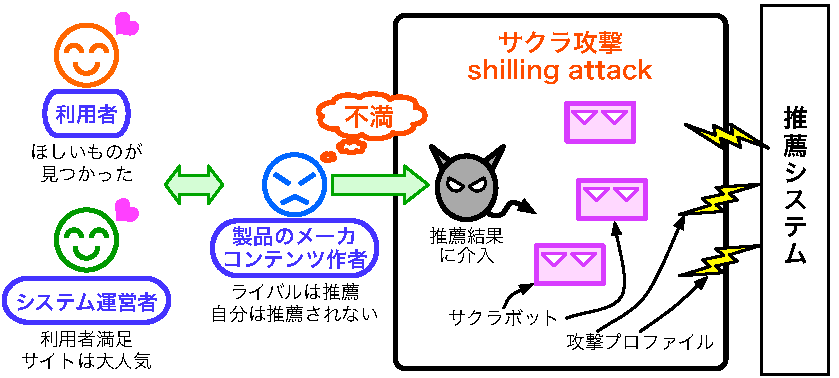
\includegraphics[width=0.96\fullwidth]{shillingattack.pdf}
\caption{サクラ攻撃を行う動機}
\label{fig:shilling-motivation}
\end{figure}

推薦システムの効用について考えてみよう(図\ref{fig:shilling-motivation}).
利用者は知りたい情報を入手できるようになり,システムに満足するだろう.これにより,システムの運営者には,システムが利用が促進されるという利点がある.
では,利用者に推薦される製品や情報の提供者にとってはどうであろうか?
自身の製品の代わりに競合他社の製品が推薦されて欲しくないとか,たとえ自社の製品が推薦されいても,さらに推薦されるよう望んだりするだろう.
これらの要求は必ずしも満たされるとは限らないため,推薦結果を自身に有利にする目的で推薦システムに干渉することが行われ始めている.
具体的な事例は\cite{www:04:01}を参照されたい.

こうした行為の一つに\term{サクラ攻撃}{shilling attack}がある.
これは,\term{サクラボット}{shilling bot} と呼ばれるエージェントプログラムや,雇った人間に,自身に有利な推薦が他の利用者になされるように,推薦システムへ嗜好データを入力させるものである.
サクラ攻撃は,利用者にとっては不適切な推薦がなされるため望ましくない.運営者にとってもシステムへの信頼を失わせる行為であるため,サクラ攻撃は排除すべきものである.
サクラ攻撃の有効性の検証や,攻撃検出などの対策は,文献\cite{jacm:04:02,www:04:01}などによって研究が始められた.
サクラ攻撃全般についてのよいまとめとしては文献\cite{ieeem:07:07}がある.
以下,サクラ攻撃の構成要素,攻撃戦略の体系的な分類,攻撃への対策を紹介する.

\section{サクラ攻撃の基本}
\label{sec:shilling:basics}

サクラ攻撃の基本事項をまとめる.
攻撃意図とは,攻撃の実行者が推薦をどのように変化させたいかという目的である.
\begin{description}
 \item[販促攻撃 (push attack)] 本来なら推薦されないはずの,自社の製品などのアイテムを推薦されるようにする.
 \item[排除攻撃 (nuke attack)] 本来なら推薦されるはずの,他社の競合製品などのアイテムを推薦されないようにする.
 \item[攪乱攻撃 (random attack)] 予測精度を下げさせて,システムへの信頼を失わせる.
\end{description}
このうち前者二つの攻撃目的について研究がなされている.
こうした攻撃は,一部の限定された利用者やアイテムに対して集中的に行われる.

一般に,大量の情報,またシステムに密接な情報を利用した攻撃ほど効果的な攻撃が可能になる.
特に,利用者の嗜好データに完全にアクセスできると,検出はほぼ不可能である.
しかし,この種の情報は,プライバシー保護の観点からも秘匿されて管理されているため,攻撃者が合法的に入手するのは困難である.
比較的容易に合法的に入手できるデータとして,アイテムへの平均評価値がある.
これらのデータを公開しているシステムや,利用者そのものでなくても,コメントを付けている編集者や利用者の評価の平均値を出しているものは多い.
さらに映画におけるIMDB~\cite{url:021}のように,アイテムの評価サイトから,代替情報を別途入手できる場合もある.
また,推薦アルゴリズムごとに効果的な攻撃の作戦があるので,推薦に用いているアルゴリズムの情報も重要である.
一時的な推薦を,協調フィルタリングで行うには,アイテム間型のメモリベース手法が多用されるといったことを用いて,この情報もある程度推定できる.

サクラ攻撃の効果は次のような指標によって測る.
\begin{description}
\item[予測シフト (Prediction Shift)] 攻撃の前後での,予測評価値の変化の全標的アイテム(後述)と全利用者についての平均.予測評価値自体がどれくらい攪乱されたかを測るための指標である.
\item[ExpTopN(Expected Top-N Occupancy)] 上位N個の推薦アイテムに標的アイテムが含まれる個数の,全利用者についての期待値.評価値が変化しても,アイテムの順位に影響するとは限らないので,実際の推薦リストの変化を測るための指標である.
\end{description}

\section{サクラ攻撃の種類}
\label{sec:shilling:tactics}

\begin{figure}
\centering
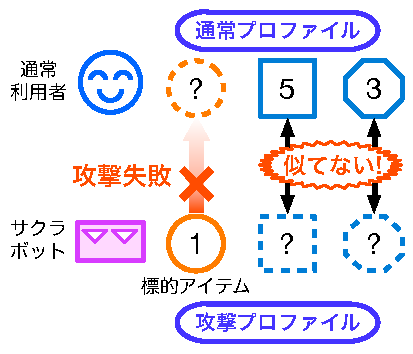
\includegraphics[width=0.6\fullwidth]{attackprofile1.pdf}\\
(a)~標的アイテムのみ\\
\bigskip
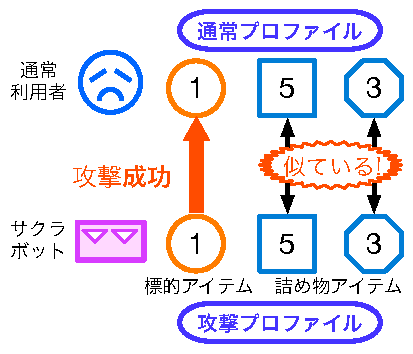
\includegraphics[width=0.6\fullwidth]{attackprofile2.pdf}\\
(b)~標的アイテム+詰め物アイテム
\caption{攻撃プロファイル}
\label{fig:attackprofile}
\end{figure}

サクラ攻撃をどのように行うかについて述べる\cite{www:04:01}.
図\ref{fig:attackprofile}は,排除攻撃の様子を示した.
まず,図\ref{fig:attackprofile}(a)に注目されたい.
上側は,通常利用者の嗜好データ(通常プロファイル)を示した.
この通常利用者に推薦されるアイテムを,サクラ攻撃によって変えたいとする.
一方,下側は,仮想利用者であるサクラボットが推薦システムに入力する嗜好データで,攻撃プロファイル (attack profile) と呼ぶ.
図中には,丸,四角,八角で示した三つのアイテムがあり,各プロファイル中では,これらのアイテムは5段階で評価されている.
「5」が最高評価,「1」が最低評価,そして「?」が未評価を示している.
この中で,丸で示したアイテムは,排除したい競合製品を表し,これを標的アイテム (target item) と呼ぶ.
通常利用者はこの標的アイテムを未評価で,今からこの利用者の標的アイテムへの評価値を予測するとしよう.

このとき,標的アイテムを推薦されないようにするには図\ref{fig:attackprofile}(a)のように,サクラボットは標的アイテムに最低の評価「1」を与えさえすれば良さそうである.
しかし,この攻撃は失敗する.多くのサクラボットが悪い評価を与えることで,このアイテムへの平均的な評価は確かに低下する.
だが,協調フィルタリングでは,嗜好パターンが似ている利用者を参考に推薦することを思いだされたい.
この利用者の通常プロファイルでは,標的アイテム以外の四角や八角のアイテムも評価されている.
一方,攻撃プロファイルでは,丸の標的アイテムのみが評価され,それ以外の四角や八角のアイテムは全て未評価である.
そのため,通常プロファイルと攻撃プロファイルは似ていないと判定され,サクラボットとこの利用者の嗜好パターンは違うとみなされる.そのため,標的アイテムの評価は通常利用者の推薦には反映されず,攻撃は失敗する.

そこで,他の利用者の嗜好パターンに攻撃プロファイルを似せるため,図\ref{fig:attackprofile}(b)のように,標的アイテム以外の四角や八角のアイテム群にも評価値を与える.
これらのアイテムを詰め物アイテム (filler item) と呼ぶ.
これらの,詰め物アイテムへの評価が通常利用者のそれと類似していれば,通常プロファイルと攻撃プロファイルとは類似していると判断される.
すると,攻撃プロファイルの標的アイテムへの評価は,通常利用者の推薦に影響し,攻撃は成功する.
しかし,通常利用者の嗜好データは入手できない.
よって,詰め物アイテムの評価値は,通常利用者の,一般的な評価の傾向に基づいて与える.
この与え方の違いによって,次のような攻撃方法がある.
\begin{description}
\item[サンプリング攻撃 (sampling attack)]
詰め物アイテムに,システムのデータベースからサンプリングしてきた評価値を与える.統計的手法では検出は不可能と言って良いが,システム内のデータベースの情報の入手は非常に困難である.
\item[ランダム攻撃 (random attack)]
ランダムな評価値を,詰め物アイテムに与える\cite{www:04:01}.必要な情報はないが,あまり効果はなく発覚し易い.
\item[人気商品攻撃 (bandwagon attack)]
良く売れている人気商品の評価は高いことが多く,また多くの利用者が評価している.
のことを利用し,人気商品に高い評価値を与えて,攻撃プロファイルの他の利用者への類似性を高める\cite{jacm:04:02}.
\item[平均攻撃 (average attack)]
詰め物アイテムに,それらのアイテムへの評価値の平均値を与える\cite{www:04:01}.
アイテムへの平均評価値は入手が比較的容易だが,利用者間型のメモリベース手法には効果的である.
一方,アイテム間型では,予測シフトで評価すると確かに評価値には影響するが,推薦リスト中でのアイテムの順位を変えるまでにはいたらず, ExpTopNへの影響は限定的である.
\item[探査攻撃 (probe attack)]
ダミー利用者を作り,その利用者に推薦されたアイテムの予測評価値を詰め物アイテムへの評価値とする\cite{ieeem:07:07}.
ダミー利用者と類似した嗜好の利用者にのみ有効な攻撃である.
\item[セグメント攻撃 (segment attack)]
映画のジャンルなど,アイテムの分類情報が利用できる場合の販促攻撃に用いる\cite{icdm:05:06}.
標的アイテムと同じセグメント(分類カテゴリ)のアイテムには,高い評価を与える.
同じセグメントのアイテムには,同じような評価がなされやすいという傾向を使う.
アイテム間型のメモリベースに対して有効な攻撃である.
\item[愛憎攻撃 (love/hate attack)]
排除攻撃専用の手法.標的アイテムには最低の評価を,詰め物アイテムには最高の評価を与える\cite{kdd:06:01}.
単純な攻撃だがアイテム間型と利用者間型のどちらのメモリベース手法についても効果がある.
\end{description}
%他の利用者がまだあまり評価していない,新規のアイテムについては,サクラ攻撃には特に脆弱である.
%現在のところ,モデルベース型の協調フィルタリングについては,まだこれらの攻撃の効果は研究が進んでいない.

\section{サクラ攻撃に対する防御}
\label{sec:shilling:defence}

作為的な利用者の評価に影響されて,協調フィルタリングが不適切な推薦をしたとしよう.
そして,他の利用者がその推薦に従ったとしても,その後,作為のない評価をするので,自律的にこうした攻撃は無力化されるとも考えられていた.
しかし,Cosleyら\cite{sigchi:03:02}はこれに対して否定的な調査結果を報告している.
以前に評価したことのあるアイテムについて,以前と同じ,1段階良い,1段階悪いの3種類のものを「予測評価」と偽って利用者に提示した.
すると,作為的にずらした方向に,アイテムへの利用者の評価が変化した.
さらに,未評価のアイテムについて,アルゴリズムができるだけ正確に予測した評価,それより1段階良い/悪い評価を利用者に提示すると,やはり,同様の傾向がみられた.
このように,心理学における同調 (conformity)~\cite{jb:026:00}と類似した,周りの意見に利用者の意見が『引きずられる』現象が報告されている.
そのため,サクラ攻撃に対して推薦システムは自律的に回復することはできず,攻撃を検出して排除する必要がある.

サクラ攻撃は,サンプリング攻撃以外は,真のデータベースの評価値分布と,攻撃プロファイルとの統計的な分布の差をはずれ値検出の技術によって見つけることで検出する.
文献\cite{sigir:06:01}の方法は,最も基本的なもので,モデルから予測される評価値と,実際の評価値の差が標準偏差に対して十分に大きければ攻撃とみなす.
ランダム攻撃は比較的に容易に検出できるが,平均攻撃では失敗することも多い.
また,サクラボットが評価するアイテム数が少ない場合や,標的アイテムが多い場合は検出が困難になると報告している.
文献\cite{kdd:06:01}では,アイテムに対する平均的な評価からの乖離を,被評価数などで加重した統計量や,ボットの攻撃は多数のアイテムに対して行われることを利用した統計量を提案している.
加えて,平均攻撃など特定の攻撃に対する検出方法も検討している.
その他,攻撃が特定の時期にまとまって行われることが多いことを利用し,時系列中での検出を試みる研究\cite{kdd:06:03}もある.
これは,あるアイテムについての評価値を,一定間隔の期間ごとに分ける.
そして,各期間内の評価値の平均やエントロピーが異常値になることを検定により検出する.
文献\cite{sigir:08:04}はサクラ攻撃に対して頑健な,行列分解を用いた推薦アルゴリズムを提案している.
この方法では,評価値行列を因子に分解するときに,利用者側の因子はそのまま計算するが,評価パターンが他の利用者と大きく異なっている疑わしい利用者の因子を利用せずにアイテム側の因子を計算する.
